\section{Results}
\label{sec:results}

\subsection{Power Comparisons}
\label{sub:power_comparisons}

Figure~\ref{fig:simulatedGeneRealData} displays the mean empirical power for each test under various scenarios for the 50 randomly selected genes.
In each scenario I considered a single causal region of size $\gamma$.
The size of the causal region was defined relative to the total gene size.
For example, given a gene with 10 rare variants and $\gamma=0.2$ then the first $2$ mutations defined as causal mutations.
Empirical power was compared between SKAT, SKAT-O, KS, burden (CMC, BURDEN) and KS-Burden under different assumed effect sizes ($r^2=(0.002, 0.006, 0.009)$).

First of all, all tests are affected by the size of the causal cluster.
As expected, KS and Skat greatly lose statistical power when $\gamma$ increases.
The KS test showed greater statistical power between $\gamma=0.3$ and $\gamma=0.6$ than Skat, but KS suffers from a lose of power in situations in which $\gamma$ is very small (10\%).
Further, the simple KS test performs better than SkatO at $\gamma=0.4$.
Both burden tests (CMC and Burden) show an monotonic increase in statistical power given an increase in $\gamma$.
In addition, omnibus tests, that is SkatO and KS-Burden, are relatively unaffected by a change in $\gamma$, but KS-Burden seems to perform worse in simulations when $\gamma$ is small.
Thus reflecting estimated statistical power of the KS test.

Overall, KS-Burden is able to outperform SkatO across all but one simulation scenario.
In scenarios in which all variants are disease causing both burden tests outperform all remaining tests.
Further, CMC and Burden seem to be equivalent in most circumstances.

\begin{figure}[ht!]
  \centering
  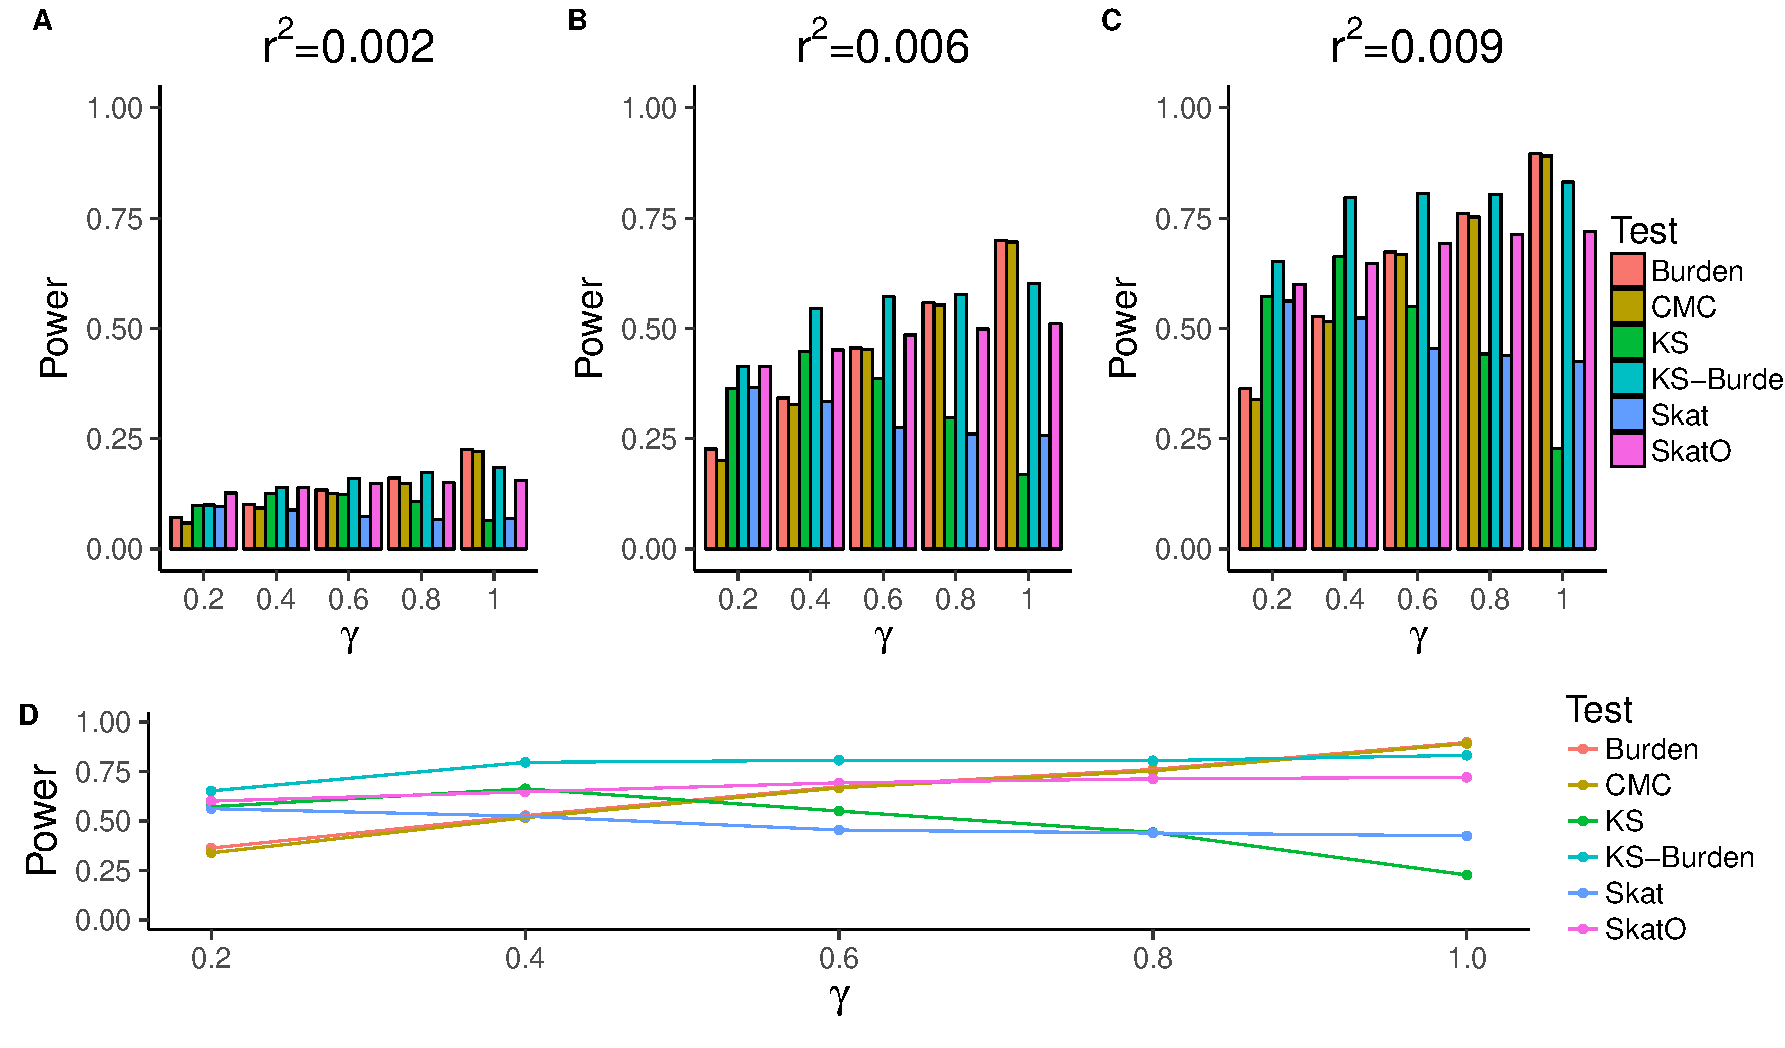
\includegraphics[width=0.8\linewidth]{figures/combined_power_analysis.pdf}
  \caption{Estimated mean statistical power for five different causal cluster size $\gamma$ over selected 50 genes.
    (A-C) display the different power estiamtions for each rare variant association test for $r^2=0.002, 0.006, 0.009$.
    The percentage of causal mutations $\gamma$ are on the corresponding x-axis, while empirical power is on the y-axis.
    (D) Relative change in empirical power over changes in $\gamma$ for each assessed test.\label{fig:simulatedGeneRealData}}
\end{figure}

\subsection{Relationship between KS and Burden}
\label{sub:relationship_between_ks_and_burden}

As described in the previous section we aimed to investigate the relationship between the KS and Burden test.
The Figure~\ref{fig:correlation_ks_burden} displays the relationship among the test statistics of both tests within all tested genes.
As one can see there seems to be no relationship between the two tests under the null of both tests.

\begin{figure}[ht!]
  \centering
  \includegraphics[width=0.8\linewidth]{example-image-a}
  \caption{Correlation between test statistics of KS and Burden under the Null across selected genes.
    No obvious correlation pattern can be detected.}\label{fig:correlation_ks_burden}
\end{figure}

Inspection of the type 1 error rate also suggests no major violations of the KSBurden test.

\subsection{UKBioBank -- Aggression}
\label{sub:ukbiobank_aggression}

Next I applied the KSBruden test on the UKBioBank data.
Specifically I investiaged distrivutional differences of rare variant across cases and controls.
The QQ-plot for all tests is displayed in Figure~\ref{fig:qqplot_ksburden} and the top $10$ genes are shown in Table~\ref{tab:top_ksburden}.


